A partir de la potencia solar instalada queremos llegar al dato de cuánta
potencia eléctrica se produce a lo largo del año, porque la potencia instalada
representa el máximo extraíble, pero esta se verá reducida con pérdidas y
niveles de radiación inferiores al máximo de diseño.

Para ello utilizamos el software SAM \cite{SAM2023} (System Advisor Model)
desarrollado por el NREL, usando los datos meteorológicos para el año 2022 que
procuramos en la sección \ref{sec:temperatura_ambiente}.

Inicializamos un proyecto fotovoltaico con modelo PVWatts, para $1[kW]$ de
paneles montados en tejado con orientación fija, inversor de eficiencia 0.96, y
otros parámetros dejados por defecto (figura \ref{fig:sam_solar_parameters}).

\begin{figure}[h] \centering
	\centering
	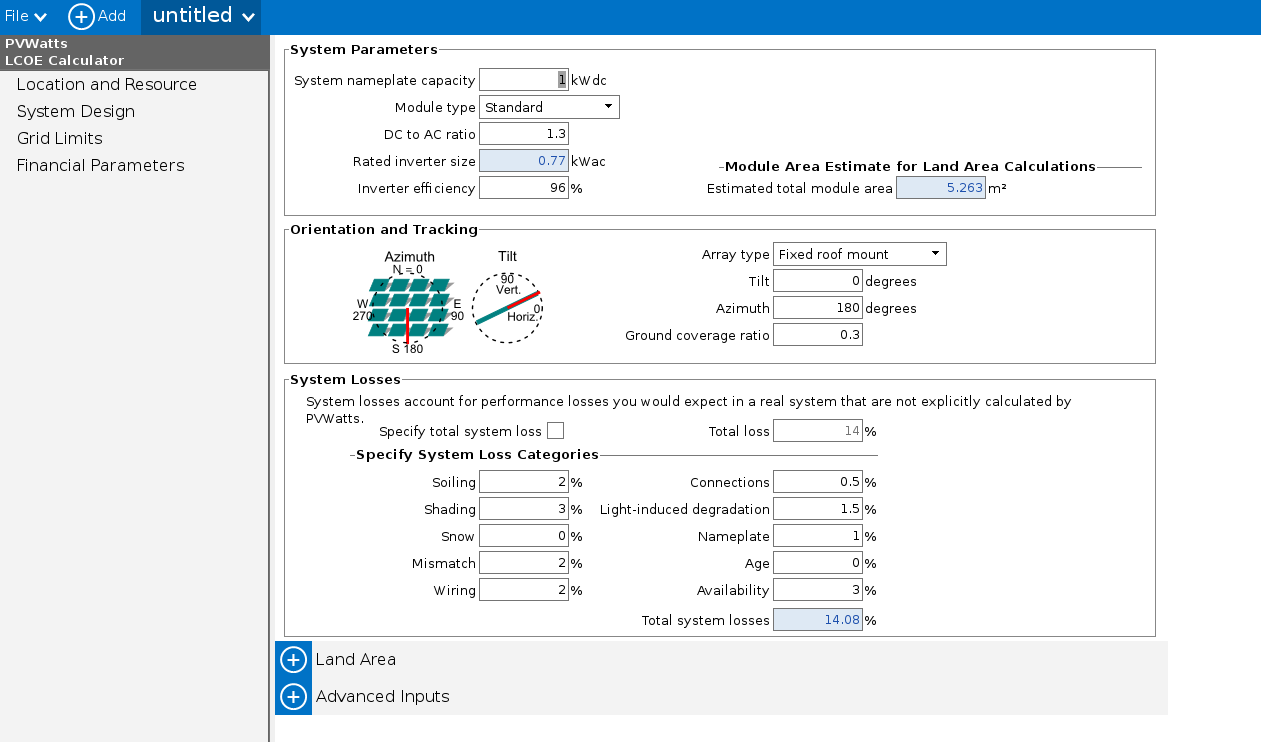
\includegraphics[width=1\textwidth]{./capitulos/adquisicion_de_datos/images/sam_solar_parameters.png}
	\caption{Parámetros para sistema fotovoltaico en SAM.}
	\label{fig:sam_solar_parameters}
\end{figure}

Tras simular el sistema, nos queda la siguiente producción solar (gráfica
\ref{fig:solar_production}).

\begin{figure}[h] \centering
	\centering
	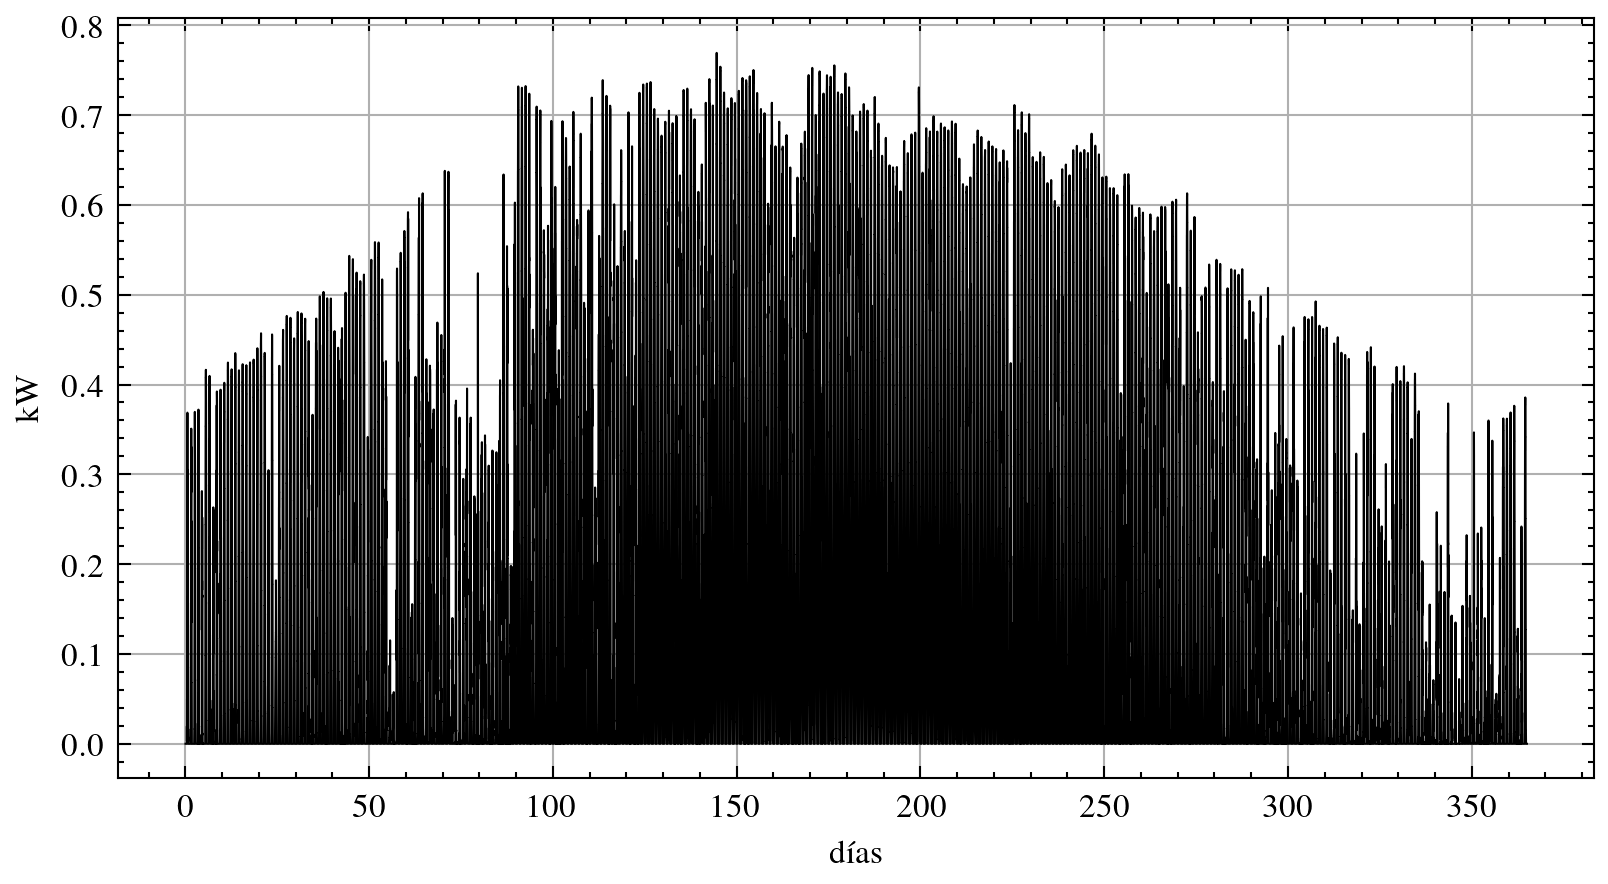
\includegraphics[width=1\textwidth]{./capitulos/adquisicion_de_datos/images/solar_production.png}
	\caption{Potencia eléctrica generada por un 1kW de paneles solares a lo largo
		de 2022 en Madrid.}
	\label{fig:solar_production}
\end{figure}
